\documentclass[fleqn,10pt]{wlscirep}
\usepackage[utf8]{inputenc}
\usepackage[T1]{fontenc}
\usepackage{algorithm,algpseudocode}
\usepackage{mathtools}
\usepackage{epstopdf}
\usepackage[justification=justified,
	format=plain]{caption}
\epstopdfDeclareGraphicsRule{.tif}{png}{.png}{%
	convert #1 \OutputFile         
}
\DeclarePairedDelimiter\ceil{\lceil}{\rceil} 
\title{Pattern matching based denoising for images with repeated sub-structures.}

% Keywords command
\providecommand{\keywords}[1]
{
	\small	
	\textbf{\textit{Keywords---}} #1
}

\author[1,*]{Anil Kumar Mysore Badarinarayana}
\author[1]{Christoph Pratsch}
\author[2]{Thomas Lunkenbein}
\author[3]{Florian Jug}
\affil[1]{Hemholtz-Zentrum Berlin, X-ray microscopy, Berlin, 12489, Germany}
\affil[2]{Fritz Haber Institute, Department of Inorganic Chemistry, Berlin, 14195, Germany}
\affil[3]{Fondazione Human Technopole, Computational Biology, Milan, 20157, Italy}


\affil[*]{anil.mysore\_badarinarayana@helmholtz-berlin.de}

%\affil[+]{these authors contributed equally to this work}

%\keywords{Keyword1, Keyword2, Keyword3}

\begin{abstract}
	In electron microscopy, obtaining low noise images is often difficult especially when examining biological samples or delicate materials. Therefore, the suppression of noise is essential for the analysis of such noisy images. State of the art image denoising methods are dominated by supervised Convolution Neural Network (CNN) based methods. However, supervised CNNs cannot be used if a noise-free ground truth is unavailable. To address this problem, we propose a method that uses re-occurring patterns in images. Our proposed method does not require noise-free images for the denoising task. Instead, it is based on the idea that averaging images with the same signal having independent noise, suppresses the overall noise. In order to evaluate the performance of our method, we compare our results with other state of the art denoising methods that do not require a noise free image. Additionally, we develop a confidence map for evaluating the denoising quality of the proposed method. Furthermore, we analyze the time complexity of the algorithm to ensure scalability, and optimize the algorithm to improve the run-time efficiency.
\end{abstract}




\begin{document}
	
	%\flushbottom
	\maketitle
	% * <john.hammersley@gmail.com> 2015-02-09T12:07:31.197Z:
	%
	%  Click the title above to edit the author information and abstract
	%
	%\thispagestyle{empty}
	
	\noindent
	\textbf{Keywords:} Image denoising, Pattern matching, Transmission Electron Microscopy
	
	\section*{Introduction}
	
	Transmission Electron Microscopy (TEM) imaging is essential in solving numerous scientific questions in life and material sciences \cite{CURRY200691}$^{,}$\cite{WANG2008395}. However, noise in the acquired images can obscure the signal. This noise can appear due to various reasons like data transmission errors and properties of the imaging systems. In addition, some noise will always be present due to the stochastic nature of the imaging process. Thus, image denoising plays a vital role especially in high resolution microscopy.
	
	The contrast in TEM imaging is based on the interaction of a multi keV electron beam with the specimen. While the optical resolution for modern TEM system can be below one angstrom,  the high energy electrons required for imaging can lead to a fast degradation of the sample. For sensitive samples, only a few electrons can be used for imaging. This leads to noisy images, thus making the image hard to interpret. Therefore, after image acquisition, numerical processing is essential to enhance the visibility of object structures in the image.
	
	In order to get the best image quality with minimum dose, various image denoising algorithms were developed in the past. Conventional denoising methods like Non-Local Means\cite{bcm_nlm}$^{,}$, BM3D\cite{DBLP:journals/tip/BM3D}, etc. mostly use a statistical approach for the denoising task, whereas most modern methods that involve a deep neural network\cite{zhang2018ffdnet}$^{,}$ \cite{zhang2017beyond} require ground truth data for training. Since in most cases, very low noise electron microscopy images are not available, modern denoising methods that require clean images as ground truths cannot be used. However, there are also some deep neural network based methods that use noisy supervision\cite{DBLP:journals/corr/abs-1803-04189} and self supervision\cite{krull2019noise2void} . Although these existing methods can denoise images, they improve the denoising quality only by a relatively small margin for images with repeated patterns. To address this issue and fill this research gap, a new denoising algorithm which effectively denoises TEM images with repeated patterns is proposed. In  our method, we also show that the fine structures in TEM images can be restored most effectively while maintaining image sharpness. In the following sections, the proposed method is explained in detail, results are analyzed and compared with the state-of-the-art methods showing significant gain in image quality. 
	
	
	\section*{Method}
	
	The proposed denoising algorithm identifies similar patches within the entire image and averages them to suppress the noise. Since the noise is assumed to be randomly distributed with zero mean, it partially cancels out when multiple patches are averaged. However, the base signal remains the same throughout and averaging does not change the signal. Hence combining different patches results in a denoised image, closer to the actual signal value. 
	
	Let $x_{i}$ be the $i^{th}$ noisy patch, $k$ be the number of patches that are averaged, $s_i$, and $n_i$ be the signal and noise in the $i^{th}$ patch respectively. Then,
	\begin{equation}
		x_i = s_i + n_i
	\end{equation}
	Averaging over $k$ patches results in an expected value,
	\begin{equation}
		E\left[\frac{1}{k}\sum_{i}^{k}x_i \right] = E\left[\frac{1}{k}\sum_{i}^{k}(s_i + n_i) \right]
	\end{equation}
	Since the noise is expected to have zero mean and the base signal is expected to be the same, this ideally means that,
	\begin{equation}
		E\left[\frac{1}{k}\sum_{i}^{k}x_i \right] = s
	\end{equation}
	In addition, variance is 
	\begin{equation}
		Var\left[\frac{1}{k}\sum_{i}^{k}x_i \right] = \frac{1}{k^2 -1} \sum_{i}^{k}Var\left[n_i\right]
	\end{equation}
	since $Var[s_i] = 0$ for all $i$. Hence averaging patches with the same signal suppresses noise.
	

	
	%The basic idea of the algorithm can be compared with the Single Particle Imaging \cite{bhushan_single_2017}, which is an image processing technique used to analyze low dose Transmission Electron Microscopy (TEM) images of identical but dose sensitive samples. Images of specimens obtained from TEM are often very noisy, and hence it is difficult to interpret the information contained in the image. Averaging several images of the same specimen can remove random noise and make the information more interpretable \cite{bhushan_single_2017}.
	
	%It can also be said that this algorithm is similar to the Non-Local Means \cite{bcm_nlm} algorithm in some aspects. In Non-Local Means, similar patches are found only from the immediate surroundings, where as the region of interest is not restricted in the proposed denoising algorithm. Increasing the search space in Non-Local Means has a massive impact on the computation speed. 
	
	\subsection*{Outline of the proposed algorithm}
	
	\begin{figure}[H]
		\centering
		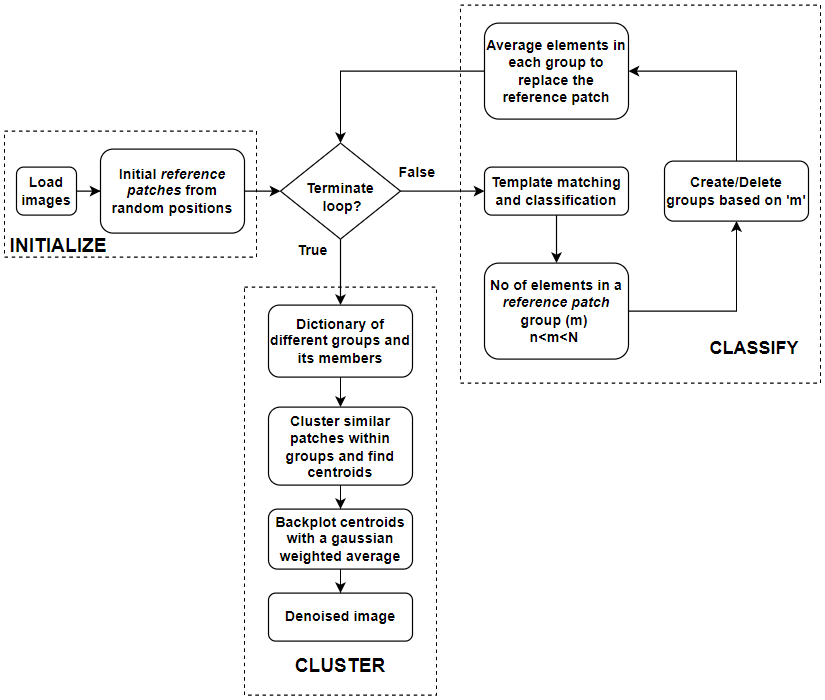
\includegraphics[scale=0.7]{./imgs/flowchart.png}
		\caption{ The proposed algorithm is depicted in this flowchart. It begins by randomly selecting patches from the noisy input image, which serve as templates for subsequent pattern matching. In the `classify' section, an iterative pattern-matching process is employed to group similar patches together, with further splitting of the group based on it's size and averaging of the group members to reduce noise. Despite this noise reduction, artifacts may persist when the group has a large variance, which is why the algorithm includes a `cluster' section to refine the groups formed. This step prioritizes grouping of the most similar patches, resulting in a seamless, artifact-free image. It is worth noting that the algorithm strategically incorporates pattern matching before clustering to minimize computational overhead, ensuring an efficient denoising process.}
		\label{fig:flowchart}
	\end{figure} 
	
	The proposed algorithm groups similar patches at two levels. Cosine similarity is used to broadly group similar patches within an image and later, clustering is used to more finely group closely matching patches within the groups obtained during the first step. A flowchart of the algorithm is shown in figure \ref{fig:flowchart} and the two levels of the algorithm are represented by `classify' and `cluster' sections of the flowchart.
	
	Cosine similarity  measures similarities between two vectors\cite{alake_understanding_2021} by finding the cosine angle between them. If the vectors are in the same direction (i.e., similar), cosine similarity is maximum. It is mathematically represented as,
	\begin{equation}
		sim(A,B) = cos(\theta) = \frac{A\cdot B}{\|A\|\|B\|} = \frac{\sum_{i=1}^{n}A_i B_i}{\sqrt{\sum_{i=1}^{n}A_i^2}\sqrt{\sum_{i=1}^{n}B_i^2}}
	\end{equation}
	where $A$ and $B$ are two vectors, and $\theta$ is the angle between them. Cosine similarity between a template and different patches of an image results in an array whose values lie between -1 and 1. Values close to the maximum represent the patches similar to the template.  Hence, cosine similarity can be used to match two image patches by considering them as vectors.
	
	%\begin{figure}
	%	\centering
	%	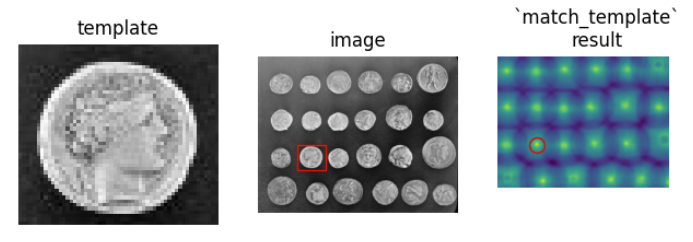
\includegraphics[scale=0.8]{./imgs/template_matching.png}
	%	\caption[Template matching example]{Template matching example \footnote{\footnotemark} }
	%	\label{fig:template_matching}
	%\end{figure} 
	
	%\footnotetext{\url{https://scikit-image.org/docs/dev/auto_examples/features_detection/plot_template.html}}
	
	


	The algorithm begins with the initialization of random patches of size $m*m$, which are used for matching other patches of the same size in the image. The patches that are used as templates for matching are referred to as \textit{reference patches}. One example for the initial choice of \textit{reference patches} can be seen in figure \ref{fig:initial_reference_patches}. 
	
	
	
	% In the `classify'  section shown in figure \ref{fig:flowchart}, the patches at every position in the image are classified into different groups based on their similarity to the \textit{reference patch} using cosine similarity. When cosine similarity is applied, each patch of size $m*m$ in the image is compared with all the \textit{reference patches}. The result has values between -1 and 1 as the results are normalized. The location with a perfect match is represented by value of 1 and patches similar to the \textit{reference patch} are represented by values close to 1. 
	
	
	In the `classify' section shown in figure \ref{fig:flowchart}, the patches at every position in the image are classified into different groups based on their similarity to the \textit{reference patch} using cosine similarity. When cosine similarity is applied, each patch of size $m*m$ in the image is compared with all the \textit{reference patches}. Local maxima are found from each cosine similarity result, which corresponds to the best fitting positions for that particular \textit{reference patch}. These resulting arrays from different \textit{reference patches} are stacked together and the maximum along the new dimension corresponds to the best fitting \textit{reference patch} for different locations of the image. Now, that the patches in the image which are most similar to the \textit{reference patches} are identified, they can be grouped together.
	
	\vspace{1cm }
	
	\begin{figure}[H]
		\centering
		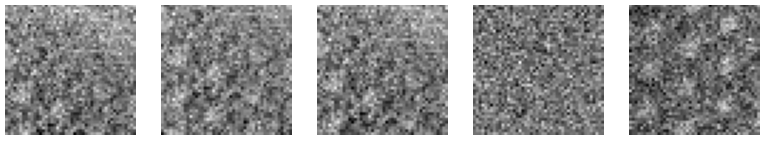
\includegraphics[scale=0.85]{./imgs/initial_reference_patches.png}
		\caption{Example set of initial \textit{reference patches} (of size $48*48$ pixels), taken from different regions of the input image. These are the first set of patches that are used as templates for pattern matching in the proposed algorithm. These raw image patches show little to no structure and the noise in these patches is dominant. }
		\label{fig:initial_reference_patches}
	\end{figure} 
	
	\begin{figure}[H]
		\centering
		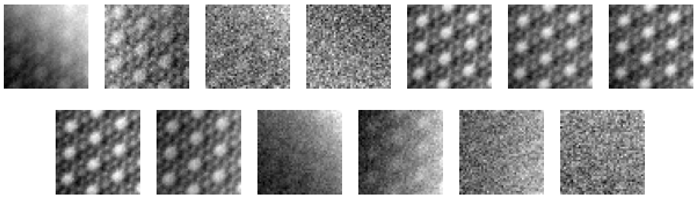
\includegraphics[scale=1.2]{./imgs/final_reference_patches.png}
		\caption{Example subset of the final \textit{reference patches} (of size $48*48$). These are also the patches obtained after the `classify' section of the flowchart shown in figure \ref{fig:flowchart}. The noise suppression in these images is already evident upon comparing these images with the initial \textit{reference patches} in figure \ref{fig:initial_reference_patches}.}
		\label{fig:final_reference_patches}
	\end{figure} 
	
	Some of these groups formed can sometimes have large number of patches in the same group, while others may contain very few unique patches. Groups with few members contribute little to the denoising, while overly large groups might lead to a loss of detail. Hence, the groups formed are deleted or split into finer groups based on the group size. Finally, for each new group, the old \textit{reference patch} is replaced by the average of all the members in that group. In the next iteration, cosine similarity and the classification steps repeat with these new \textit{reference patches}. When the classification becomes stable, there are no new groups formed. This is when the iteration loop is broken. Figure \ref{fig:final_reference_patches} shows the \textit{reference patches} generated after 15 iterations. On comparing figure \ref{fig:initial_reference_patches} and figure \ref{fig:final_reference_patches}, one can observe that the noise in the final \textit{reference patches} has been significantly suppressed.


	
	If the final \textit{reference patches} are directly used for back-plotting (i.e. to replace the patches from their corresponding positions in the image), there would still be some artifacts present. This could arise sometimes because image patches that are not similar to any of the \textit{reference patches} end up falling into the best available group, even though the group might not be their best representation. This is required since the entire region of the image has to be covered. When outliers are included during averaging, the mean deviates from the median signal value. Additionally, the unique features present as outliers will be lost in the averaging process, both of which are undesirable. Another reason for artifacts is that, cosine similarity is only sensitive to the structure for any two patches and ignores the offset (i.e. brightness). Therefore back plotting might not recover local brightness variations.
	
	These problems can be solved by averaging over a small group with very closely matched patches. To achieve this, clustering is applied within every group (represented by the final \textit{reference patch}) to create smaller subgroups. The number of clusters in a group can be adjusted by a user set parameter. In other words, the target signal-to-noise ratio can be adjusted by changing this parameter value. While previously the whole group was represented by a single \textit{reference patch}, it is now represented by centroids of the subgroups after clustering. Centroids are back-plotted with a $2D$ Gaussian weighted average. These Gaussian weights smooth the edges of the centroids, thus preventing artifacts in the reconstructed image. 
	
	A pseudo implementation of the algorithm is shown in the additional information section. The implementation of the denoising algorithm can be found on github (\url{https://github.com/mbanil/img-denoiser}).
	
	\subsection*{Parameters of the algorithm and stability}
	
	For optimal performance, the algorithm requires a few parameters which the users can tune. The parameters include size of the features defined by patch size, position of the initial patches and, depending on the amount of denoising desired, the upper and lower limit of the group size for cosine similarity classification. Finally, the group size for clustering can also be adjusted, which closely defines the desired signal to noise enhancement. If the average number of elements in a subgroup is $N^2$, there is an improvement in the signal quality by a factor of $N$ times\cite{bcm_nlm}.
	
	\section*{Results}
	
	The proposed algorithm is mainly developed to denoise TEM images with repeated structures. In figure \ref{fig:comparison} the results from all the methods and their Fast Fourier transforms (FFT) can be seen for the noisy image, . The FFT converts data from the spatial domain to the frequency domain. The signal corresponding to the low frequency components is represented at the center of the FFT and higher frequency components are present as we move away from the center. Noise corresponds to the unstructured background, as seen in the high frequency region of the FFT, and is present close to the edges.
	
	When analysing figure \ref{fig:comparison} for the noisy image, we note that it contains a lot of grainy structures which makes it hard to interpret the information. This is also reflected in the FFT, where clear structures are only visible close to the center. In figure \ref{fig:comparison}, the noisy image is followed by denoised results obtained from different methods. 
	
	N2V\cite{krull2019noise2void} is a self supervised, deep learning based image denoising method. N2V was trained with the patches of the noisy image. The training was done with $64*64$ patches, 100 epochs and a neighboring radius of 5. The results from N2V show decently reconstructed circular structures and the noise in the black region of the image has been removed fairly well. However, the substructures have not been reconstructed accurately. The FFT shows enhanced structures at the center, whereas the boundary mostly looks dark representing the suppression of high frequency noise. 
		
	BM3D \cite{DBLP:journals/tip/BM3D} is one of the widely used classical denoising methods. BM3D uses collaborative filtering in the transform domain for denoising images and it is a non-blind denoising method, which means that the standard deviation of the noise is required for denoising. The standard deviation was estimated with trial and error. We obtain the best results for a standard deviation of 0.06 for the normalized image. The result from BM3D are similar to that obtained from N2V. The denoising effect is visible but the images are still not very useful for further analysis. This conclusion is also supported by the FFT.
	
		
	Non Local Means (NLM) \cite{bcm_nlm} is a conventional image denoising method that finds similar patches of images within a region and averages them to suppress noise. An NLM implementation with a patch size of $48*48$, a search area of $100*100$ and a cut off distance of 0.36 was used. The result shows a good level of denoising. Circular structures and their subsequent substructures are generally better visible, and noise suppression is effective in most regions. But at some regions, the existence of noise can still be seen. The FFT also shows stronger structures supporting our conclusion of image feature enhancement. Overall, the results look good and more interpretable. 
	
	\begin{figure}[H]
		\centering
		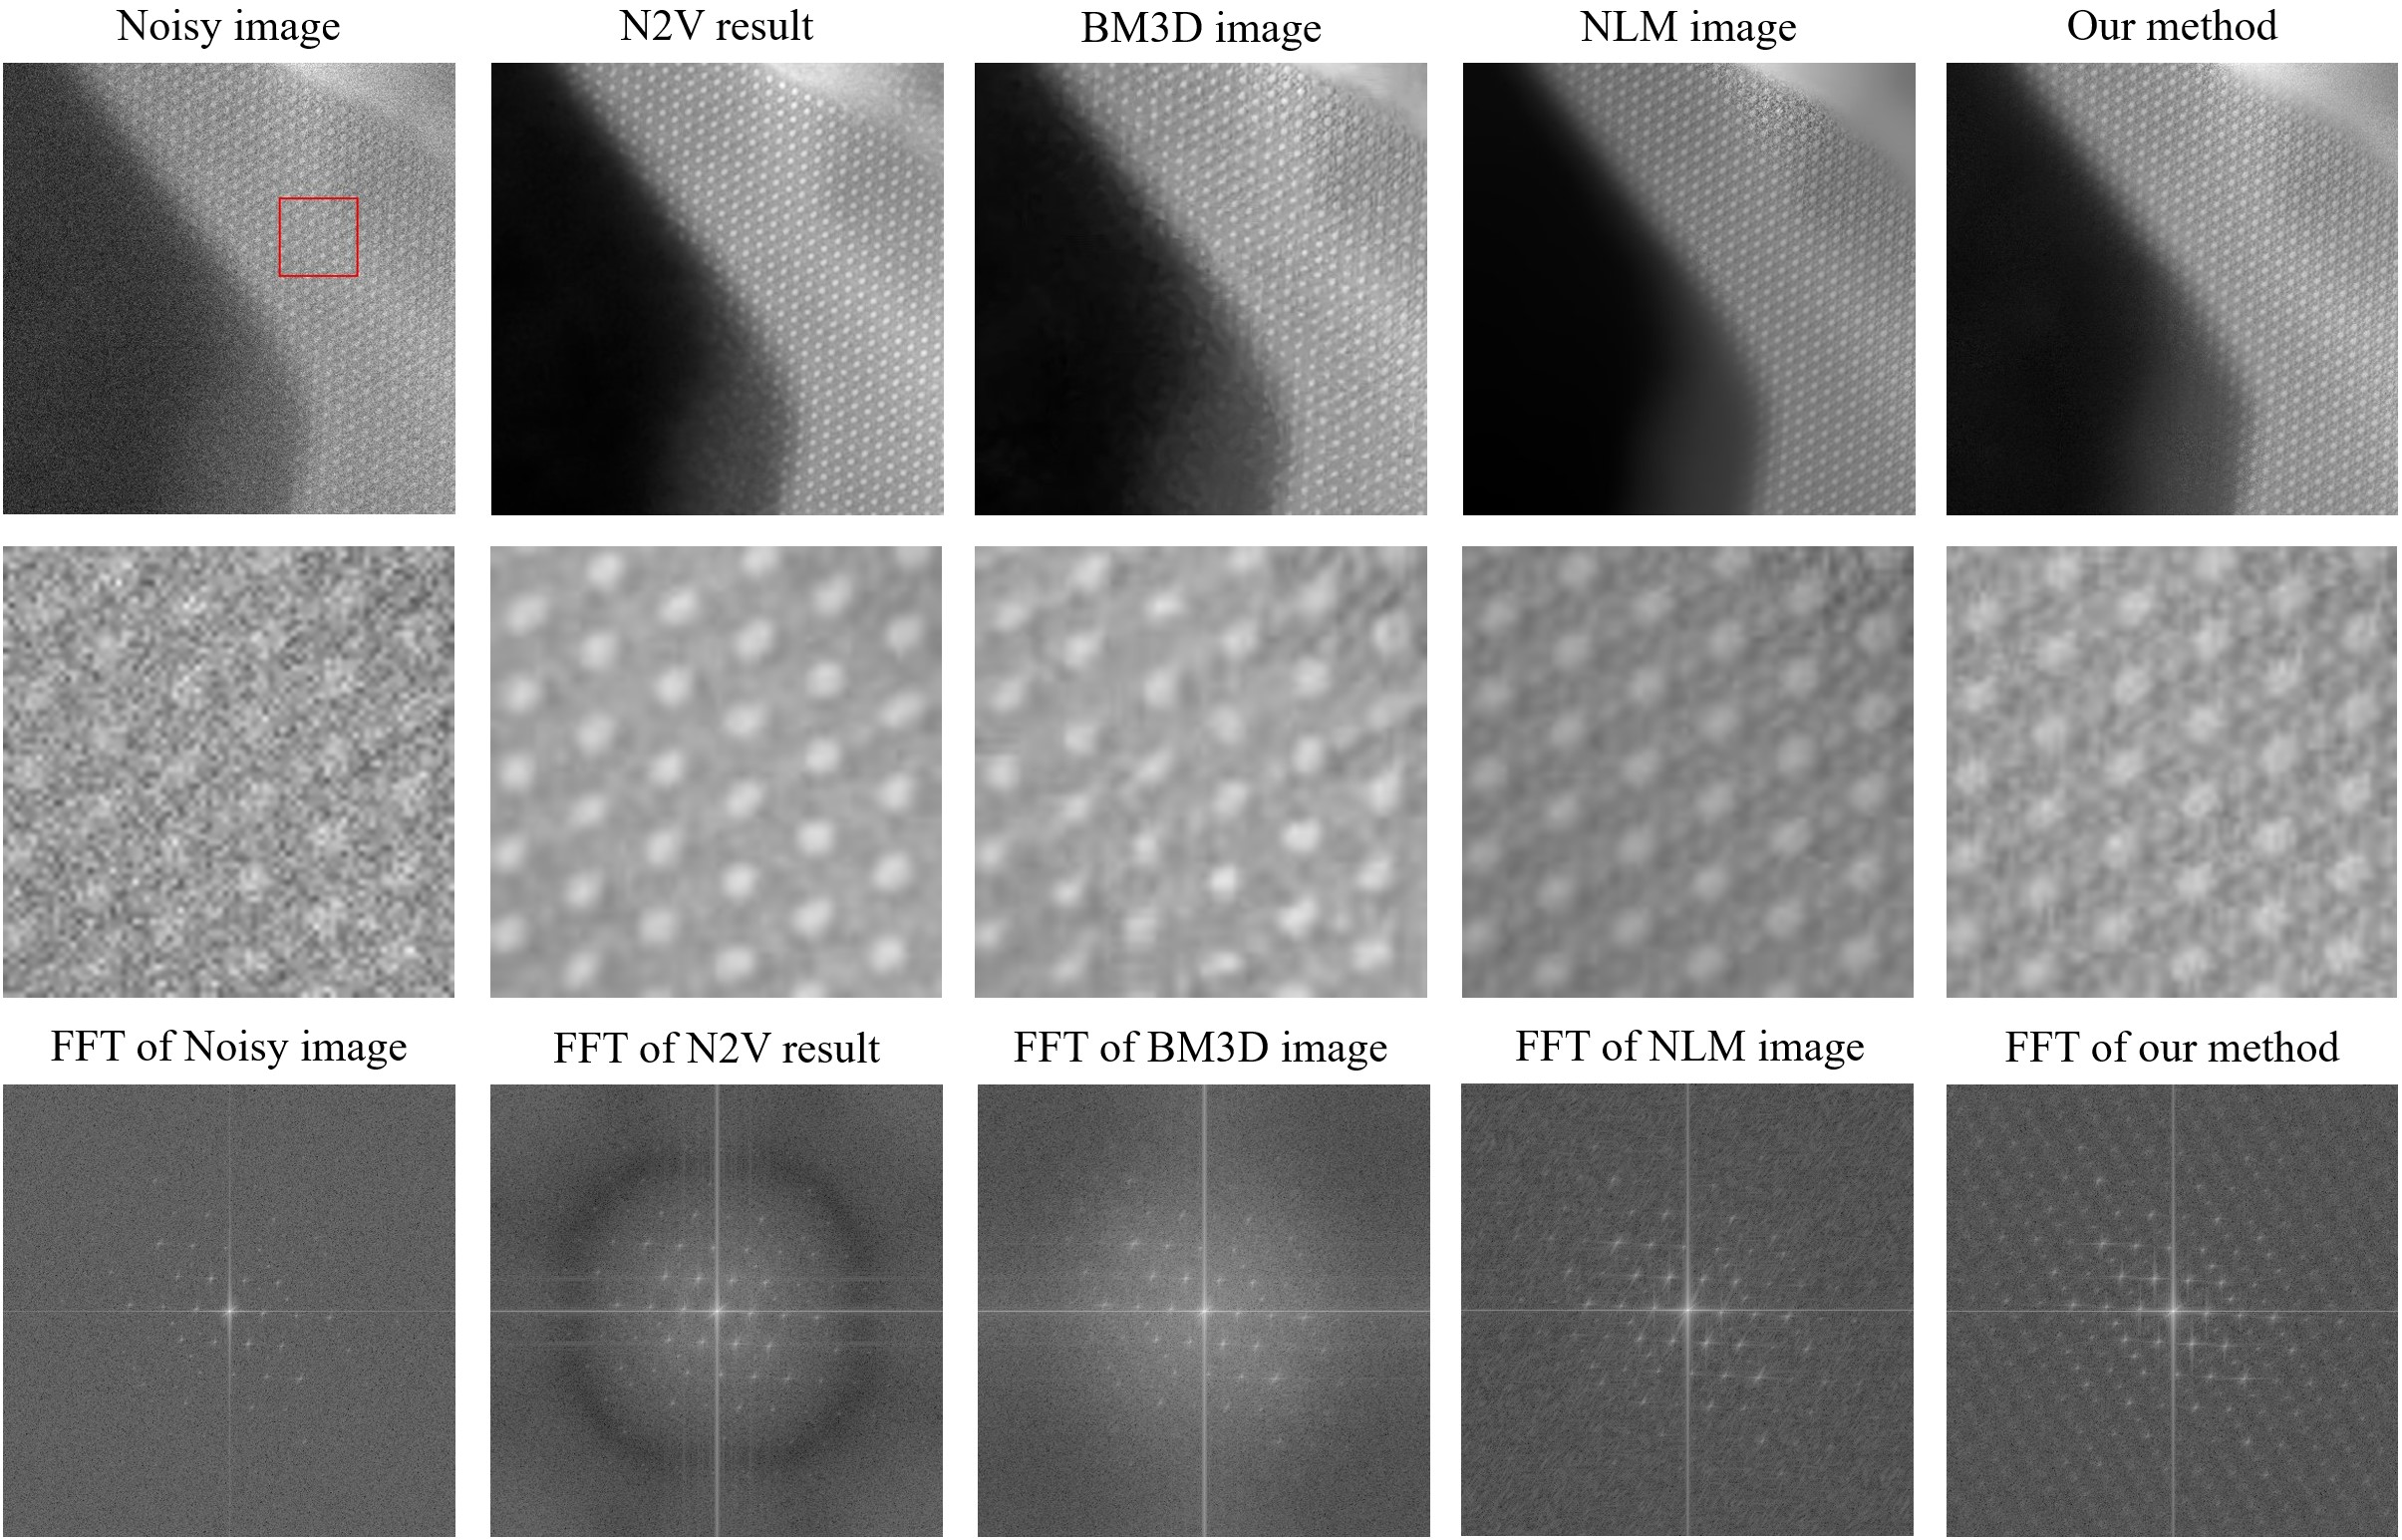
\includegraphics[scale=0.4]{./imgs/comparison-zoomed.jpg}
		\caption{First row (from left to right) shows the noisy image, and results obtained from different methods - N2V, BM3D, NLM and our proposed method. Corresponding FFTs can be seen in the second row. In the first row, insets show a zoomed-in region of the image. These insets are taken from the same location in all images and help in interpreting the denoised results better. It should be noted that, even though NLM is qualitatively close to our method, computationally it is significantly slower. }
		\label{fig:comparison}
	\end{figure}
		
	Results of our proposed denoising algorithm were obtained with a patch size of $48*48$, a group size between 5 and 100, and the clustering parameter equal to 2.7. From the denoised result, it can be observed that the quality of denoising is marginally better than that from NLM. Noise suppression is the highest compared to the other methods and information in the image can be best interpreted. The sub structures between the circular structures are also better visible. From the FFT too, we see that the structures are more prominently visible. Some features can also be seen in the high frequency region which were previously not visible so well.

	
	Apart from the qualitative improvement in the results, the proposed algorithm has a bigger advantage with regards to the computational time. The time complexity of the convolution operation is $O(m^2n^2)$, where $m*m$ is the size of the patch and $n*n$ is the size of the image, which is worse than the runtime of the template matching algorithm when $m$ is large. Complexity of the template matching algorithm is $O(n^2log(n^2))$ \cite{template_matching}, where $n*n$ is the image size. Since the convolution operation is widely used in convolution neural networks, there are Python libraries that support GPU computation for performing this operation. Running the computations on the GPU makes the algorithm significantly faster.
	
	The runtime of the proposed method for the images in figure \ref{fig:comparison} was 19.4 seconds, where as NLM, which was the closest to our results qualitatively, had a runtime of 171.4 seconds. The optimization in the runtime is particularly helpful when denoising image stacks from Transmission Electron Microscopy. The images in the stacks are often similar. In such cases, our algorithm not only matches the templates in the current image, but also the patches from other images in the stack. This significantly improves the quality of the results and with GPU computations, the computation speed is quite fast. For reference, the denoising of an image stack with 10 images of size 1024*1024 pixels took 281.8 seconds. The computations were carried out on a computer with 128 GB of RAM, Intel Xenon processor (16 CPUs), and Nvidia RTX6000 GPU. 
	
	%With the same image stack and the same computer, the computations for NLM did not terminate even after 1 hour.
	

	

	
	\subsection*{Comparison with sample images}
	
	\begin{figure}[H]
		\centering
		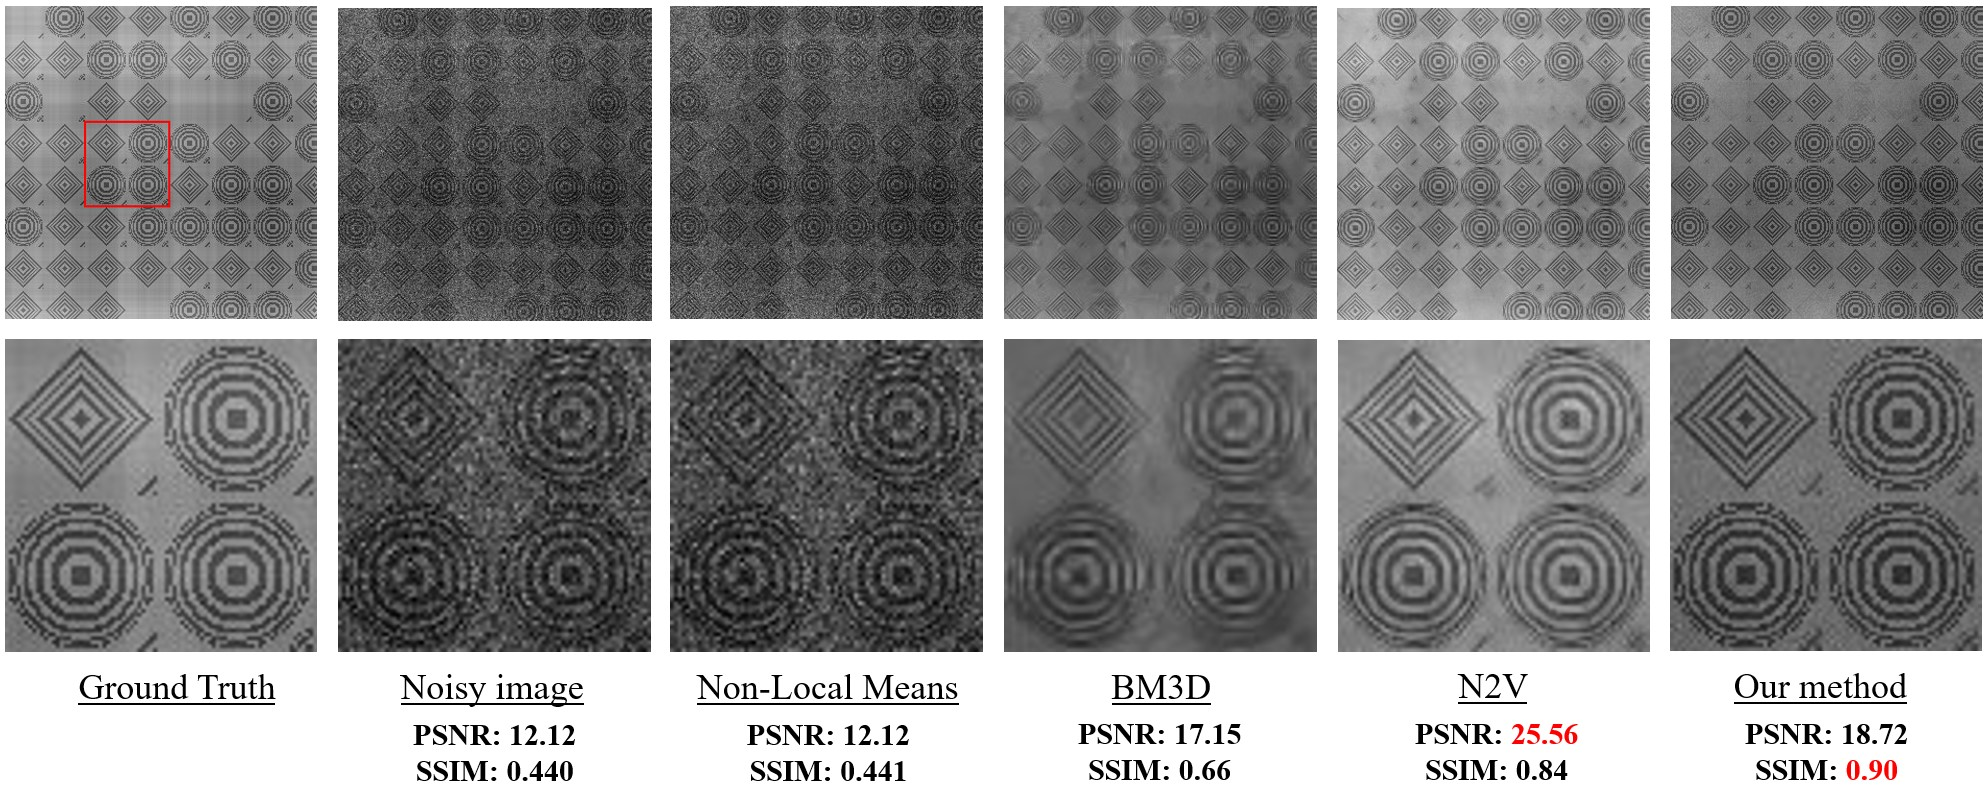
\includegraphics[scale=0.5]{./imgs/comparison_sample_new_zoomed.jpg}
		\caption{First row (from left to right) shows the simulated image (which is the ground truth), noisy image created by adding Poisson noise, and  results obtained from different methods - NLM, BM3D, N2V and our proposed method. Second row shows the corresponding zoomed-in regions images for better interpretation. PSNR and SSIM values are also shown for noisy and denoised images. N2V which optimizes for a lower distortion has a higher PSNR value. However, our proposed method succeeds in restoring high frequency components of the image. This is also supported by the fact that our method has a higher SSIM value, which is a more perceptual metric.}
		\label{fig:comparison_sample}
	\end{figure}


	Since obtaining low noise images is often very difficult in microscopy, we generated a noise free image (ground truth) artificially for quantitative comparison. The generated image tries to imitate the kind of microscopy images which are best suited for our algorithm's application, i.e. images with similar patterns spread across them. A noisy image is simulated by adding Poisson noise to the generated image. Different denoising methods were applied on this noisy image and the Peak Signal to Noise Ratio (PSNR) and Structural Similarity Index Metric (SSIM) values of the denoised images have been found with respect to the ground truth. The ground truth, noisy image and the results from different methods can be seen in figure \ref{fig:comparison_sample}. Additionally, a comparison of the FFT of these images is shown in additional information section.
	
	The results from Non-Local Means show minimum improvement. The reason is that this method requires similar image patches that are present close to each other, which is not always the case in the generated image. BM3D processes the image in the Fourier domain and hence suppresses the high frequency components. This results in the sharp features of the image being less prominent. N2V does a better denoising job which is reflected in its PSNR value. However, on close inspection it can be observed that the high frequency components appear slightly blurred. This is where our method out-performs the others. The pattern matching used to find similar pattern across the image ensures the correctness while preserving the sharpness of the image. This is also reflected in a higher SSIM value.
	
	It should be noted that PSNR is based on mean squared error and is a distortion based evaluation metric. In image restoration there is always a trade-off between the distortion and the perceptual quality of the restored image. Often it is not possible to achieve both simultaneously \cite{8578750}. As shown in figure \ref{fig:comparison_sample}, we obtain the best results with our method for SSIM which is a more perceptual metric, although we do not achieve the best PSNR value \cite{8578750}.
	
	\subsection*{Confidence map}
	
	\begin{figure}
		\centering
		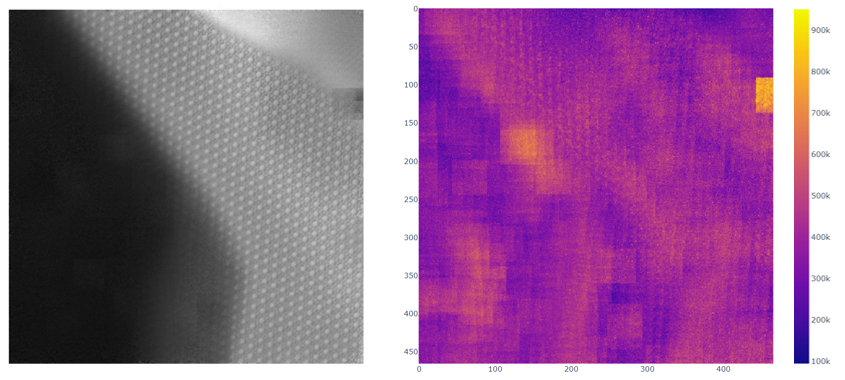
\includegraphics[scale=0.7]{./imgs/confidence_map.png}
		\caption{An image denoised by using our proposed method (left) and it's confidence map (right) can be seen in the figure above. When patches are averaged, the variance of the group is also found along with the average. The variance calculated is used to back-plot at the corresponding location in a weighted manner to get the confidence map. Ideally, the variance should be minimum. High variance regions show strong deviations and the presence of dissimilar patches in the same group. Such high frequency regions lead to the creation of artifacts. An example of such an artifact can be identified by the bright yellow regions on the confidence map.}
		\label{fig:confidence_map}
	\end{figure}
	
	In the absence of a ground truth, it is difficult to identify artifacts in the denoised results. However, it is essential to recognize these artifacts to prevent incorrect interpretations of the denoised images. Since it is challenging to detect minute artifacts from FFT, a confidence map is developed. This confidence map is based on the variance within each cluster obtained after applying clustering. The idea behind this approach is that the variance should be small if the centroid is a good representation of its members. Also, a good centroid should not have any patterns in its variance. Patterns in the variance therefore show that the centroid does not generalize its members well. 
	
	The confidence map of the denoised image is calculated by combining the variances\cite{chan1982updating} for different centroids as they are back-plotted. The overall variance map, i.e., the confidence map of a denoised image is shown in figure \ref{fig:confidence_map}. This result has been produced for demonstration purposes with a very few initial \textit{reference patches} selected very close to each other. The bright regions in the confidence map correspond to the denoised image artifacts. For instance, a bright region can be seen in the confidence map at the top-right position. An artifact can be found by inspecting the same region in the denoised image. Similarly, irregularities in the black region on the left side of the denoised image can be recognized by the brighter regions of the confidence map.
	

	
	\section*{Discussion}
	
	Denoising of the experimental images obtained from electron microscopy was performed by using popular denoising methods - N2V, BM3D and NLM. Even though these methods successfully suppressed noise, they enhanced fine image features only by a small margin. To address this problem, a new denoising algorithm was developed which makes use of similar patterns present in images and averages them to suppress noise. This new method successfully denoises images and also enhances fine structures. The results of all the denoising methods are compared using FFT. Additionally, a confidence map is developed to evaluate the denoising results when ground truth data is absent. Quantitative comparison of the denoising results is done using an artificially generated image. The quantitative comparison demonstrates the ability of our proposed method to preserve high frequency components in images.  
	
	The time complexity of the algorithm was analyzed. Optimizations were made to enhance the computation speed by introducing cosine similarity instead of template matching. This helped in enhancing the run-time efficiency by a significant factor, which ensures scalability.
	
	\bibliography{sample}

	%\section*{Acknowledgements (not compulsory)}
	
	%Acknowledgements should be brief, and should not include thanks to anonymous referees and editors, or effusive comments. Grant or contribution numbers may be acknowledged.
	
	\section*{Author contributions statement}
	
	A.K.M.B implemented and optimized the algorithm, C.P conceptualized the idea, the experimental images were taken by T. L, and F.J reviewed the work technically by providing feedback whenever required.  All authors reviewed the manuscript. 
	
	\section*{Additional information}
	
	\subsection*{FFT comparison of the sample images}
	\label{fftcomparison}
	
	\begin{figure}[H]
		\centering
		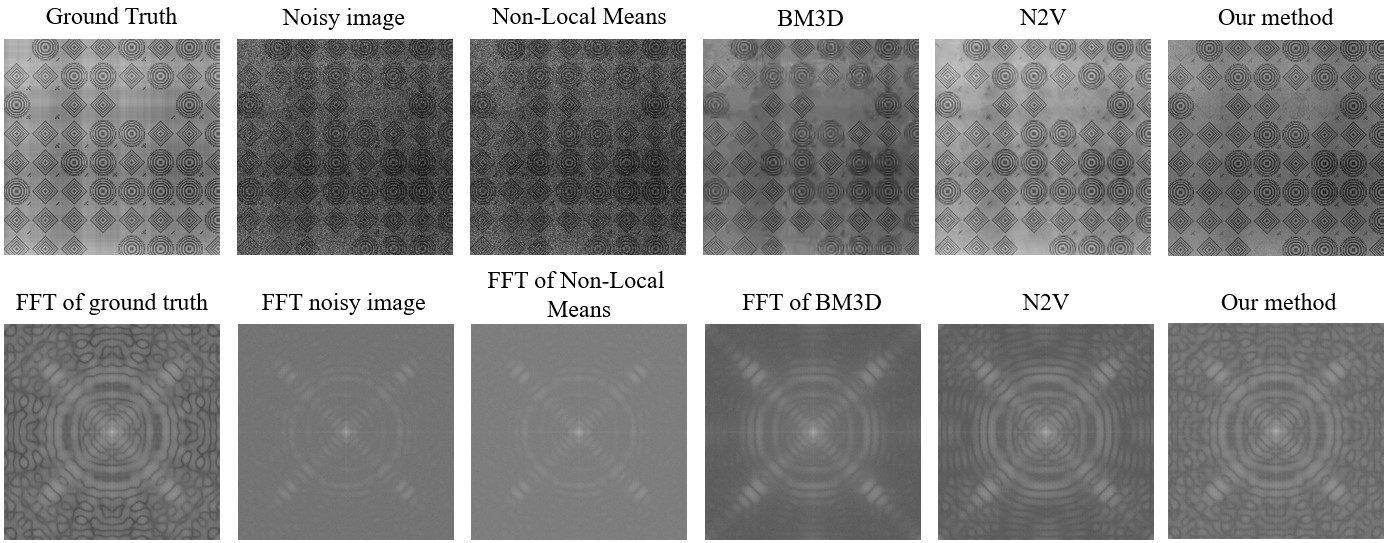
\includegraphics[scale=0.6]{./imgs/comparison-sample_fft.jpg}
		\caption{First row (from left to right) shows the simulated image (which is the ground truth), the noisy image created by adding Poisson noise, and the results obtained from different methods - NLM, BM3D, N2V and our proposed method. Corresponding FFTs can be seen in the second row. Close inspection of the FFTs shows that our method comes closest to the ground truth.}
		\label{fig:comparison_sample_fft}
	\end{figure}

	In addition to the quantitative comparison of different denoising algorithms for the artificially generated image, an FFT comparison is shown in figure \ref{fig:comparison_sample_fft}. The fine details are not visible on the FFTs for the images denoised using Non-Local Means and BM3D. The FFTs of these images show only small improvements compared to the FFT of the noisy image. The FFT of the image denoised with N2V shows finer details. However, the FFT of the image denoised with our method shows the most details compared to the others. The FFT from our method is also the one closest to that of the ground truth. This clearly shows that our method outperforms the other methods in image restoration, while preserving the fine details of the image. 
	
	\subsection*{Algorithm}
	\label{algorithms}
	
	\begin{algorithm}
		\caption{Denoising Algorithm}
		\label{algorithm:denoising_algorithm}
		\begin{algorithmic}[1]
			\State \textbf{Input}: Noisy image (\textit{imgs})
			\State \textbf{Result}: Denoised image
			\State set [\textit{templateSize, minGroupSize, maxGroupSize, clustParam, loopTermination}] ;
			\State \textit{refPatches} $\gets$ generate\_initial\_ref\_patches(\textit{imgs}, \textit{templateSize}) ;
			
			\For{\textit{loopTermination} $\geq$ 0 \textbf{or} (check if the number of \textit{refPatches} in the last two iterations has changed)}
			
			\State \textit{tmpMatchResult} $\gets$ [ ]	;		
			
			\For{\textit{img} in \textit{imgs}}
			\For{\textit{refPatch} in \textit{refPatches}}
			
			\State \textit{tmpMatchResult}.append(template\_matching(\textit{img}, \textit{refPatch})) ;
			
			\EndFor
			\EndFor
			
			\State \textit{maxValue} $\gets$ max(\textit{tmpMatchResult}, axis=2) ;
			\State \textit{refPatchIndex} $\gets$ `\textit{refPatches}' index at \textit{maxValue} ;
			\State [\textit{sorted\_maxValue, positionX, positionY}] $\gets$ sortWithIdx(\textit{maxValue}); 
			\State \textit{t} = \textit{templateSize} ;
			\State \textit{list[\textit{idx},\textit{posX},\textit{posY}]} = [ ];
			%%		\algstore{part1}
			%%\end{algorithmic}
			%%\end{algorithm}
			%%\begin{algorithm}
			%%	\begin{algorithmic}[1]
				%%		\algrestore{part1}
				
				\For{each \textit{s,posX,posY} in \textit{sorted\_maxValue, positionX, positionY}}
				\If{\textit{maxValue[posX,posY]} \textbf{not equal} 0}
				\State \textit{maxValue}[\textit{posX: posX}+($t/4$); \textit{posY: posY}+($t/4$)] $\gets$ 0 ;
				\State \textit{idx} $\gets$ \textit{refPatchIndex}[\textit{posX},\textit{posY}] ;
				\State \textit{list}.append([\textit{idx},\textit{posX},\textit{posY}]) ;
				\EndIf
				\EndFor
				
				\State [\textit{count,refPatchID}] $\gets$ count\_patches\_with\_same\_id(\textit{list});
				% \State \textit{max\_ind} = max(\textit{refPatchIndex}) ;
				
				\For{\textit{cnt,ID} in \textit{count,refPatchID}}
				\If{\textit{cnt} $\le$ \textit{minGroupSize}}
				\State \textit{list} $\gets$ delete(\textit{list}, \textit{ID});
				
				\ElsIf{\textit{cnt} $\ge$ \textit{maxGroupSize}}
				
				\State \textit{list} $\gets$ splitGroup(\textit{list}, \textit{ID}, \textit{maxGroupSize});
				
				%\For{\textit{l} in \textit{list}}
				%	\If{list[idx] == ind}
				%		\If{loopCounter == \textit{params}[\textit{maxGroupSize}]}
				%			\State \textit{loopCounter} = \textit{loopCounter} + 1
				%			\State \textit{list}[\textit{idx}] $\gets$ \textit{max\_ind}
				%			\State \textit{max\_ind} $\gets$\textit{ max\_ind} + 1
				%		\EndIf
				%	\EndIf
				%\EndFor
				
				\EndIf
				
				\EndFor
				
				\State \textit{refPatches} $\gets$ average\_patches\_with\_same\_id(\textit{list}) ;
				
				\State \textit{loopTermination} $\gets$ \textit{loopTermination}-1 ;
				\EndFor
				\State \textit{subGroup}[\textit{centroid, posX, posY}] = [ ];
				\For{\textit{refPatchID} in \textit{refPatches}}
				\State \textit{patches\_with\_sameRef} $\gets$ get\_patches\_with\_same\_id(\textit{list},\textit{refPatchID});
				\State \textit{numClusters} $\gets$ count(\textit{patches\_with\_sameRef})/\textit{clustParam} ;
				\State \textit{subGroup}.append(cluster(\textit{patches\_with\_sameRef, numClusters})) ;
				\EndFor
				\State \textit{gaussianWeight} $\gets$ createGaussianWeight();
				\State \textit{denoisedImg} $\gets$ backPlot(\textit{subGroup}, \textit{gaussianWeight});
			\end{algorithmic}
		\end{algorithm}
		
%		\clearpage
		
		%\begin{algorithm}
		%	\caption{Algorithm for calculating variance}
		%	\label{algorithm:variance_algorithm}
		%	\begin{algorithmic}[1]
			%		\State \textit{weight} $\gets$ \textit{weightA} + \textit{weightB} ;
			%		\State \textit{delta} $\gets$ \textit{avgB} - \textit{avgA} ;
			%		\State \textit{M2} $\gets$ (\textit{M2\_A} + \textit{M2\_B} + $delta^2$ *  \textit{weightA} * \textit{weightB}) / n ;
			%		\State \textit{Var\_AB} = \textit{M2} / (\textit{n} - 1);
			%	\end{algorithmic}	
		%\end{algorithm}
		
			

		
	\end{document}